\chapter{Command Arbitration for Modular Reinforcement Learning}\label{ch:arbiq}

In this chapter we demonstrate the performance degradation of modular reinforcement learning agents whose module have incomparable reward scales. Arrow's Impssibility Theorem for social choice provides an explanation for the failure of existing approaches to modular reinformcent learning and a framework for our solution. We present our solution, the Arbi-Q command arbitration algorithm, and empirically demonstrate that it does not exhibit the same performance degradation as existing approaches to modular reinformcement learning.

\section{Modular reinforcement learning}

In the previous chapter we explained the state of the art in modular reinforcement learning as a decomposition of an implicitly global Q-function in to additive modules. To support software engineering we would like these components to be truly modular. In particular, we would like the components to be reusable and easily understood by agent authors.  Unfortunately, current approaches implicitly require a global, monolithic reward signal, which detracts from these properties.  In particular, it detracts from the ability of the agent author to locally define the reward for a component because the reward scales of other modules must be taken into account.

\subsection{Command Arbitration}

Like any software engineering, agent programming would benefit from modularity.  Truly modular reinforcement learning would facilitate speed of learning convergence, state abstraction, and transfer -- a module written in one context can be reused in another context because the component is dependent only on its own local reward signal.  In this section we discuss the difficulties that current approaches face in achieving true modularity and present a new formulation which solves the core problem in Section \ref{sec:mrl-solution}.

To properly investigate our proposed mechanism of combining local learners, we will restrict our attention to the MRL framework. In this framework, a learning agent, $M$, is represented by a set of $n$ subproblems (modules), $M=\{M_j\}_{j=1}^n$, each having its own reward signal and state space. The typical formulation is to have subproblems share an action set, thus $M_j = (S_j,A,R_j)$. When the agent takes an action in the world, each subproblem's state is updated, and each subproblem receives a reward. The agent can be thought of as having a state space that is a cross product of the subproblem state spaces, $S=S_1\times S_2\times\ldots\times S_n$. Equivalently, each module can be considered to have a state space that is a subset of the global state space -- a module state that is an abstraction of the world state. Traditionally, it is assumed that the agent's reward is a sum of subproblem rewards, $R(s,a)=\sum_{j\in N} R_j(s,a)$, where $N=\{1,\ldots,n\}$. Thus, $M$ is well-defined as a reinforcement learning problem, $M=(S,A,R)$, and the goal is to find a joint policy $\pi(s)$, composed of locally learned policies $\pi_j(s)$, that is optimal for the whole agent. We let $Q_j(s,a)$ refer to the Q-value learned by component $j$ for state $s$ and action $a$. Again, traditionally, $Q(s,a)=\sum_{j\in N} Q_j(s,a)$.

\subsection{Merging local signals}

Difficulty arises when multiple single goals are being combined in a larger, multi-goal learning problem. Take AvoidWolf and FindFood for instance; it is fairly straightforward to code an internally consistent reward signal for each.  However, it is unclear how to combine the two into the larger task of LiveLong.  For example, if there is no penalty for failing to eat within a certain time period (starvation), then the obvious policy is to avoid the predator and ignore the food.  Such a degenerate case could also happen if the reward signal for one learning module were scaled without re-engineering the other reward signals in the system, a problem explained by Bhat, et., al. \cite{bhat2006on-the-difficulty}. For example, one could imagine swapping-in a new AvoidWolf module with a reward several times higher than the previous module, such that avoiding the predator always carries higher reward than finding the food.  In this case, a delegating agent would favor AvoidWolf to the near exclusion of FindFood.  The ability to substitute learning modules without modifying the rest of the system is one of the primary benefits of true modularity, and this modularity is difficult to achieve if local reward signals must be merged.

\subsection{Ideal Arbitration is Impossible}

Aside from the practical challenges cited above, Bhat, et., al.  \cite{bhat2006on-the-difficulty} showed that ideal arbitration is impossible in full generality because command arbitration reduces to Arrow's Paradox \cite{arrow1963social}: an agent is a ``society'' of modules, and command arbitration is social choice.  The problem is that we want the arbitrator to have the following reasonable properties:

\begin{itemize}

\item \textbf{Universality}: the ability to handle any possible set of
  modules.

\item \textbf{Unanimity}: guarantee that if every module prefers
  action A, so will the arbitrator.

\item \textbf{Independence of Irrelevant Alternatives}: each
  module's preference for actions A and B are independent of the
  availability of any other action C, prevents any particular
  module from affecting the global action choice by dishonestly
  reporting its own preference ordering.

\item \textbf{Scale Invariance}: ability to scale any module's
  Q-values without affecting the arbitrator's choice.  This is the
  crucial property that allows separately authored modules with
  incomparable reward signals.

\item \textbf{Non-Dictatorship}: no module gets its way all the time.

\end{itemize}

According to Arrow's Paradox, if $|A|\geq 3$, then there does not exist an arbitration function that satisfies each of the properties listed above.  So even simple agents with more than three actions are too complex for theoretically ideal arbitration.  This dissertation contributes a novel formulation of MRL and an algorithm that implements it, which we discuss in Section \ref{sec:mrl-arbiq}.

\section{Reformulating MRL}

Bhat, et., al., \cite{bhat2006on-the-difficulty} argued for a ``benevolent dictator'' arbitrator function but left the arbitration algorithm unspecified.  The contribution of this work is to show that a first-cut arbitration algorithm embodying the ideas in \cite{bhat2006on-the-difficulty} performs competitively with other MRL algorithms and shows superior robustness to module modification.  This robustness to module modification is the chief enabler of truly modular reinforcement learning in which modules can be transferred from one system to another without having to re-engineer the reward signals to fit the new host system.

In this work, we relax the dictatorship requirement in order to make a practical arbitrator-based learning algorithm feasible.  In the next section we present our Arbi-Q algorithm based on this practicalized arbitrator-based framework.

%% This is a ``fix'' because it is a reformulation. It doesn't get around
%% the impossibility result but instead defines a different thing to
%% optimize.  This fits though...now all learners are more homogenous;
%% they all have a local reward signal to optimize.

%% So while it is hard to write once-and-for-all a reward signal for a
%% multiple-goal learning problem, it is easier to write a collection of
%% single-goal reward signals, and hopefully combine them in a meaningful
%% way. Whereas in previous work, we show that there is no
%% general-purpose arbitration rule for combining subgoal preferences, in
%% the present work we make the hypothesis that the arbitrator itself is
%% a subgoal and thus has it's own notion of what it means to do its
%% subgoal well, i.e, has it's own reward signal. This means, given the
%% appropriate state, the supergoal can learn to select substeps
%% optimally. The question is what state constitutes ``appropriate
%% state''. The uninteresting case is the one in which the supergoal
%% state is simply the world state, in which case we have garnered no
%% saving, as this is simply flat RL all over again.

%In discussing MRL techniques, we will follow the nomenclature as
%introduced by ~\cite{sprague03multiple}.

\subsection{Formalization}

Our reformulation of MRL adds a {\em command arbitrator} \cite{brooks1986a-robust}.  The arbitrator has a state space that may be the same as or different from the modules' state spaces, an action set that represents choosing a module, $A_{CA} = {1 ... n}$, and a reward signal that represents the ``greater good.'' The arbitrtator's reward function, $R_a(s)$, is independently defined rather than being derived from the module rewards.  It is now another part of the problem specification; in the partial programming setting, this corresponds to $R_a(s)$ being human-authored. Note that $R_a(s)$ may or may not be equal to the sum of the rewards of the agent's modules. In fact, the module rewards $R_i(s,a)$ may not have any correlation with the arbitrator's reward $R_a(s)$.

The agent's policy is defined indirectly by the arbitrator's policy, $\pi_{CA}(s, a)$, which assigns probabilities to the selection of each module's preferred action for each state.  This formulation relaxes the non-dictatorship requirement of ideal arbitration if you think of the arbitrator as a special module.  By Arrow's theorem, other properties will still hold.

For the agent author, this formulation adds the requirement of authoring a dedicated reward signal for the arbitrator.  For our bunny agent, this is LiveLongProsper:

\begin{itemize}
\item {\em Why} avoid predator, {\em why} eat? To live longer.
\item Encodes the tradeoffs between modules -- perhaps food is more
  important to some bunnies.
\item The arbitrator could be hand-authored, or could be another RL
  agent.
\end{itemize}

For the small cost of authoring a reward signal that represents the ``greater good'' you get true modularity, that is, the ability to combine separately authored modules with incomparable rewards.  This new reward signal is now the metric we use to measure the performance of the agent.

In our MRL framework an agent is an arbitrator plus a list of modules. Formally, an agent consists of the following elements:

\begin{enumerate}
\item A reward function for the command arbitrator, $R_{CA}(s)$,
\item An action set $A$ for the agent as a whole, shared by each module,
\item A set of reinforcement learning modules, $M$
\item A state abstraction function, $moduleState_i$ for each module $m_i$
\end{enumerate}

In the next section we present a reinforcement learning-based command arbitration algorithm.

\section{The Arbi-Q Command Arbitration Algorithm}\label{sec:mrl-arbiq}

Our reformulation of MRL is based on an independently specified arbitrator \cite{brooks1986a-robust} that is itself a reinforcement learner. The state space for the arbitrator is the world state -- no state abstraction is used for the arbitrator. The arbitrator's action set, $A_{CA}$, is a set of integer indexes to the agent's list of modules (we use $CA$ in subscript to refer to the command arbitrator and numbers or $i$ to refer to modules).  As with any reinforcement learner, the arbitrator learns a policy. In the case of the arbitrator this policy, $\pi_{CA}$ is a mapping from states to modules. The modules' policies are mappings from abstracted module state to actions in the world, that is, the agent's actions. The policy defines which module chooses the agent's action in a particular state.

Arbi-Q uses a Q-Learning algorithm to learn the arbitrator's policy. At each time step the arbitrator uses its policy to select a module, then the module uses its local policy to select an action that the agent executes. The Arbi-Q algorithm is detailed in Algorithm \ref{alg:arbiq}


\begin{algorithm}
  \caption{Arbi-Q}\label{alg:arbiq}
  \begin{algorithmic}
    \State $Q_{CA} \gets$ random initial values
    \For{each module $i$}
       \State $Q_{i} \gets$ random initial values
    \EndFor
    \For{each episode}
      \State $s \gets$ world.initialState()
      \State $m \gets \epsilon-$greedy action for $s$ from $\pi_{CA}$ derived from $Q_{CA}$ \Comment{choose module}
      \State $s_{m} \gets moduleState(s)$ \Comment{abstract state for module}
      \State $a \gets \epsilon-$greedy action for $s_{m}$ from $\pi_m$ derived from $Q_m$
      \Repeat
        \State Execute $a$, observe effects $r_{CA}$ and $s'$
        \State $a' \gets \epsilon-$greedy action for $s'$ from $\pi$ derived from $Q$
        \State $Q_{CA}(s, a) \gets Q_{CA}(s, a) + \alpha [R_{CA}(s) + \gamma Q_{CA}(s', a') - Q_{CA}(s, a)]$
        \For{each module $i$}
          \State $s'_{i} \gets moduleState(s')$ \Comment{abstract state for module}
          \State $r_i \gets reward(s_i)$ \Comment{module-specific reward}
          \State $Q_i(s, a) \gets Q_i(s, a) + \alpha [r_i + \gamma Q(s_i', a') - Q(s_i, a)]$
        \EndFor
        \State $s \gets s'$
        \State $a \gets a'$
      \Until $s$ is terminal
    \EndFor
  \end{algorithmic}
\end{algorithm}

Notice that Arbi-Q is learning its command arbitration policy at the same time the modules are learning their subtasks.

\section{Experiments}

Our principal claim is that Arbi-Q is robust to modules with incomparable reward scales, which would be an authoring error in existing MRL approaches. Our experiments show that GM-Q/Q-decomposition degrades when a module is modified to have an incomparable reward scales and that Arbi-Q is robust to such modification.

\subsection{Bunny-Wolf World}

We use a world derived from Sprague and Ballard ~\cite{sprague2003multiple-goal}.  In Bunny-Wolf world, our agent is a bunny that must eat food and avoid being eaten by a wolf.  We can represent such an agent in our formulation as follows:

\begin{itemize}

\item Module 1: FindFood.  The bunny agent must find food in order
  to continue living.  If an agent does not find food within some
  number of time steps, it starves, terminating the episode.

\item Module 2: AvoidWolf.  The bunny agent must avoid the wolf.
  Meeting the wolf terminates the episode.

\item Agent's overall goal (implemented in arbitrator): LiveLongProsper.  For a given agent, being happy can mean dying young with a full stomach, or dying old but less sated.  Either conception of happiness requires the FindFood and AvoidWolf modules defined below.  The arbitrator, in a sense, encodes the agent's ``value system'' by representing the relative weight the agent assigns to its modules. To facilitate comparison to GM-Sarsa, LiveLongProsper's goal is to get as much food per time step as possible, which will require balancing food finding with wolf avoidance. This performance metric is essentially a composite of the comparably scaled modules of the GM-Sarsa agent.

\end{itemize}


We validate Arbi-Q's performance by comparing it with Greatest Mass Sarsa, which is a Q-decomposition algorithm that orders actions by their summed Q-value, $X_a=\sum_j Q_j(s,a)$. We evaluate each algorithm similarly to Sprague and Ballard \cite{sprague2003multiple-goal} by training for 100,000 time steps and evaluating performance every 10,000 steps.  Performance is evaluated by running the greedy policy in the world for 1000 episodes and calculating the average reward per episode.  Each algorithm used a discount rate of 0.9 and $\epsilon$-greedy action selection during training with $\epsilon$ linearly discounted from 0.4, as in Sprague and Ballard's experiments.

For baselines, GM and Arbi-Q algorithms used modules with similarly scaled rewards. For robustness validation, we scaled the FindFood module reward by 10 to simulate the swapping out of separately-authored learning modules.  We believe that a truly modular arbitrator function should handle such module modification without serious degradation of performance.  Otherwise, any time a learning module were modified, the arbitrator, and possibly all the other modules, would need to be modified to ensure compatibility.

\section{Results}

\begin{figure}[ht]
  \begin{center}
    \scalebox{.75}{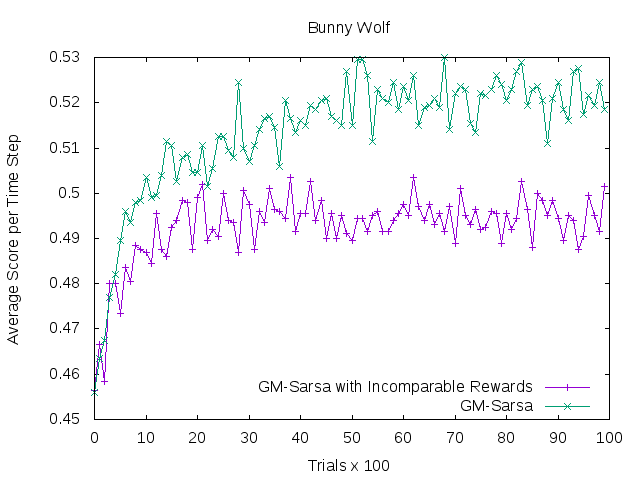
\includegraphics{gm-bunny-wolf.png}}
    \scalebox{.75}{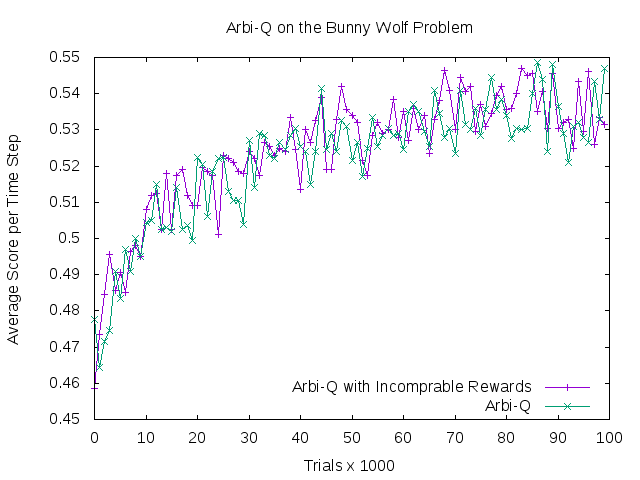
\includegraphics{arbiq-bunny-wolf.png}}
    \caption{Performance of Arbi-Q versus GM-Sarsa/Q-decomposition on the bunny-wolf problem. The top plot shows that Greatest Mass command arbitration degrades significantly when its module rewards are incomprable. Arbi-Q shows no degredation in performance when modules have incomprable rewards, suggesting that it is amenable to ``swappable'' modules.}
  \end{center}
  \label{fig:bunny-wolf-results}
\end{figure}

In


\subsection{Related Work}

Rohanimanesh and Mahadevan extended the options HRL framework to concurrent settings in which multiple agents executing multiple simultaneous actions \cite{rohanimanesh2001decision,rohanimanesh2002learning}. Their work differs from ours in that their framework applies to a single agent taking multiple actions or multiple agents taking simultaneous actions, whereas we are concerned with a single agent executing a single action that is descided by multiple reinforcement learning modules.

Marthi and colleagues \cite{marthi2005concurrent} suggest extending their work in concurrent ALisp to include the Q-decomposition algorithm of Russel and Zimdars \cite{russell2003q-decomposition}, but this line of research was not pursued. Lau and colleagues developed a modular reinforcement learning system that uses a central coordinator for multiple concurrent MPDs \cite{lau2012coordination}. Lau's work differs form ours in that they develop a constraint system in the central coordinator that limits the allowable actions of the component reinforcement learners, thereby constraining their learning. Our approach does not require the arbitrator to know details of component learners, and component learners require no explicit or implicit knowledge of the arbitrator or the other components.
